\documentclass{article}

\usepackage[T1,T2A]{fontenc}
\usepackage[utf8]{inputenc}
\usepackage[english,russian]{babel}

\usepackage{pdfpages}
\usepackage{multirow}

\usepackage{caption}

\usepackage{amsmath}
\usepackage[hidelinks]{hyperref}


\usepackage{graphicx}%Вставка картинок
\graphicspath{{noiseimages/}}

\usepackage{float}%"Плавающие" картинки
\usepackage{wrapfig}%Обтекание фигур (таблиц, картинок и прочего)

\makeatletter
\def\@biblabel#1{#1. }
\makeatother

\setlength{\emergencystretch}{10pt}

\begin{document}

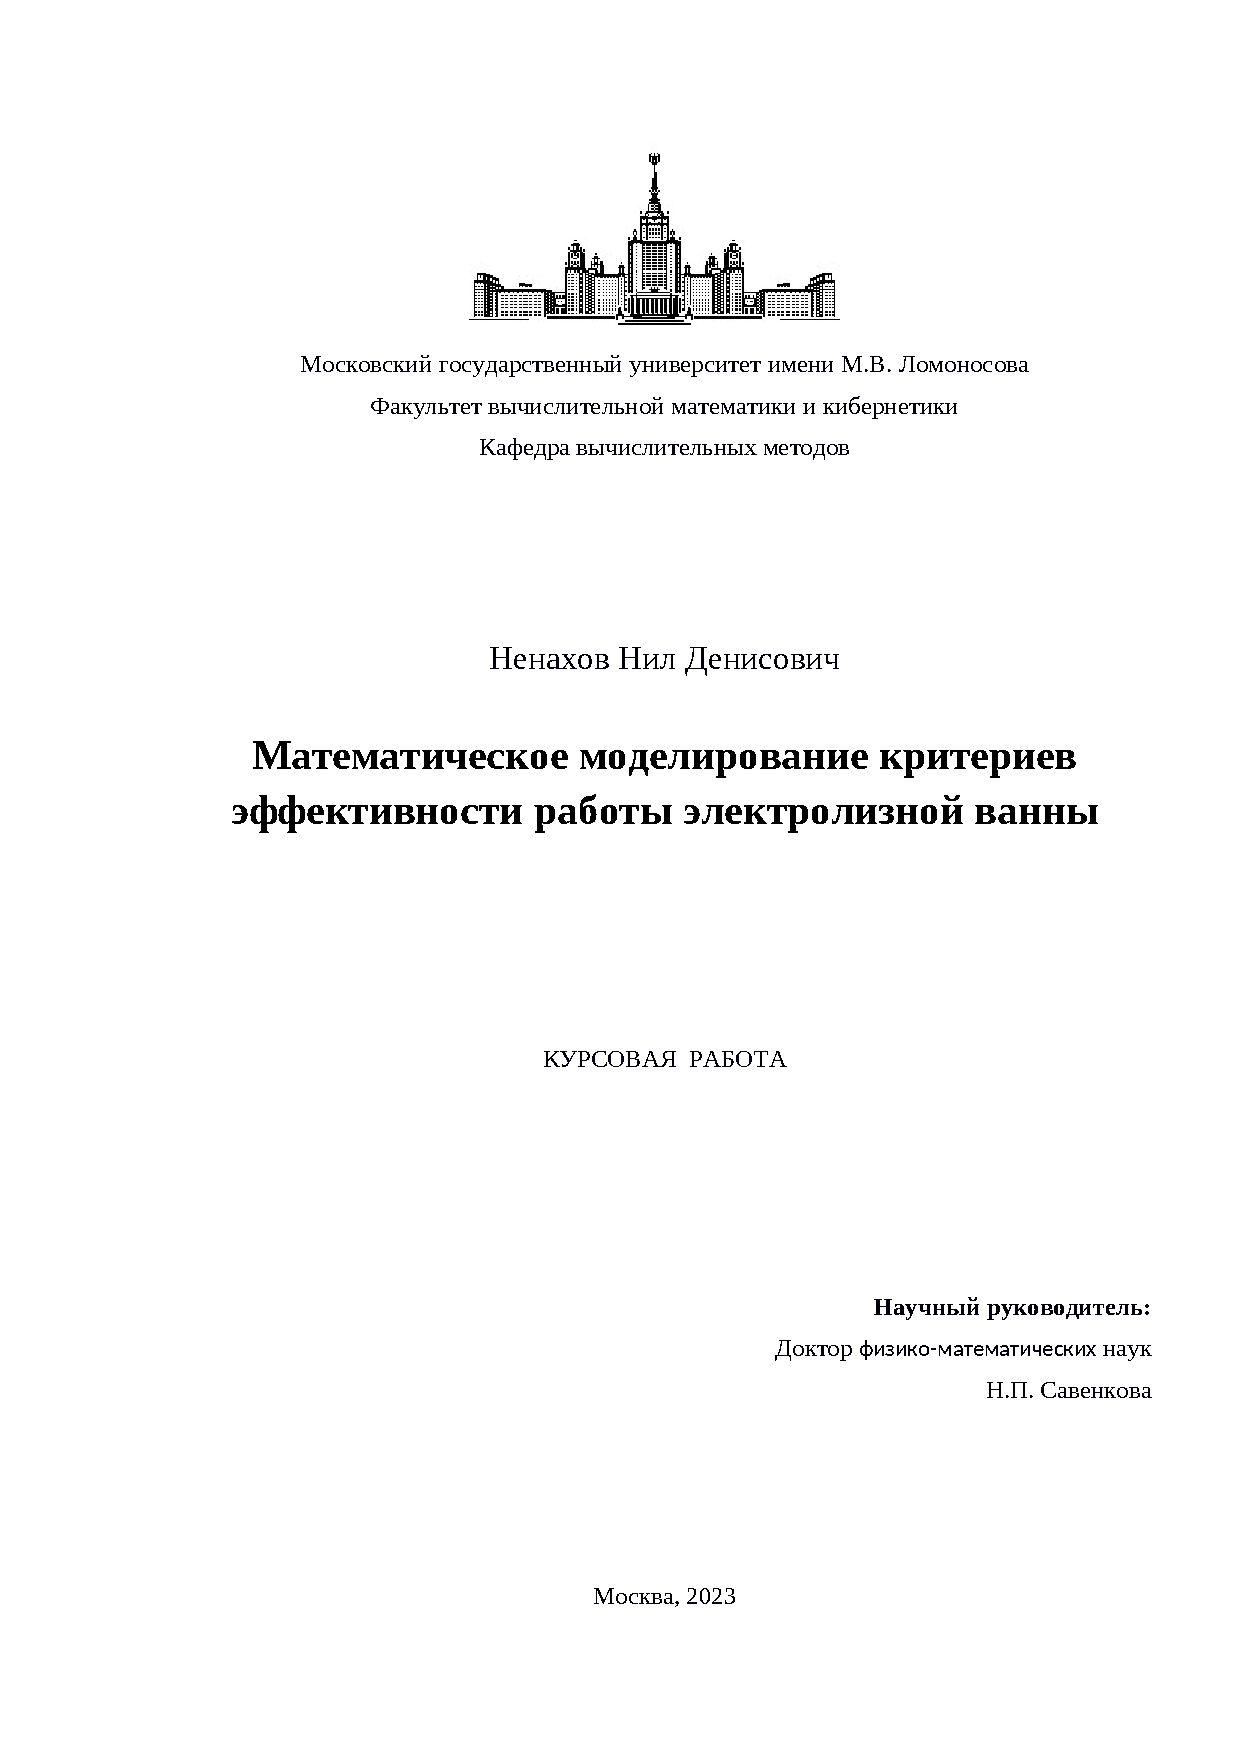
\includepdf[pages=-]{Titul.pdf}

\newpage

% переименовываем  список литературы
\addto\captionsrussian{\def\refname{Список литературы}}

\setcounter{tocdepth}{5}
\tableofcontents

\newpage

\section*{Введение.}
\addcontentsline{toc}{section}{Введение}

\subsection*{Постановка задачи.}
\addcontentsline{toc}{subsection}{Постановка задачи}

Целью исследовательской работы является проведение математического моделирования одного из основных параметров процесса промышленного электролиза алюминия - потери выхода алюминия по току.

Производство алюминия играет очень важную роль в экономике России. Процесс электролиза очень сложен, энергозатратен и серьезно влияет на экологию. Для удешевления себестоимости металла и улучшения экологичности производства имеет смысл совершенствовать не только устройство электролизера, но и способы управления процессом электролиза. С этой целью в промышленных цехах производства алюминия создаются линии АСУТП (Автоматическая система управления технологическим процессом), которые позволяют значительно повысить эффективность принятия решений при управлении процессом электролиза с целью повышения выхода алюминия и исключения негативного влияния человеческого фактора.

АСУТП, ориентируясь на значения управляющих параметров, автоматически оценивают текущее состояние процесса электролиза и принимают управляющие решения по стабилизации и повышению эффективности процесса электролиза. В силу высокой температуры и агрессивности чреды использование большинства приборов становится практически невозможно. В настоящее время рассчет управляющих параметров происходит на основе полу-эмпирических формул, в которые входят значения, которые получаются в результате физико-физических экспериментов (замеров), проводимых в реальном времени \cite{litlink:kalmykov}. В отдельных случаях некоторые химические характеристики рассчитываются на основе одномерных математических моделей, большинство которых не являются динамическими. Замер межполюсного расстояния и химический анализ состава электролита измеряется раз в две недели, поэтому АСУТП вынуждена принимать управляющие решения на основе устаревших данных по этим управляющим параметрам. Регулярно измеряются лишь насколько параметров, это сила тока и напряжение в рабочем пространстве электролизера, также могут быть измерены падение напряжения на аноде и в ошиновке \cite{litlink:bibliogr}.

Целью данной работы, является проведение математического моделирования одного из основных параметров производства алюминия - потери выхода алюминия по току в целях повышения эффективности работы АСУТП.

\subsection*{Обзор литературы.}
\addcontentsline{toc}{subsection}{Обзор литературы}

Ниже приведено краткое описание процесса электролиза алюминия и основных типов алюминиевых электролизеров \cite{litlink:bibliogr}.

Процесс получения алюминия электролизом глинозема происходит по следующей схеме. В прямоугольную ванну, футерованную углеродистым материалом, помещается слой расплавленного алюминия, над ним - слой расплавленного глинозема. В ванну опускают один анод(в случае электролизера Соделберга), через который поступает электрический ток в рабочее пространство ванны. В качестве побочного продукта образуются газы ($CO, CO_2$), которые скапливаются под анодом \cite{litlink:bibliogr}. Схема алюминиевого электролизера приведена на рисунке \ref{fig:elec}.

Электролизеры с самообжигающимся анодом (электролизеры Соделберга) имеют один анод и уступают многоанодным ваннам в производительности и экологичности. В свою очередь для многоанодных электролизеров требуются заранее изготовленные аноды, которые попарно заменяются после выработки текущих. Используемая сила тока напрямую зависит от типа и конструкции электролизера и может варьироваться от 70 кА до 400 кА при напряжении в 4-5 В \cite{litlink:bibliogr}.

\begin{figure}[H]
\centering
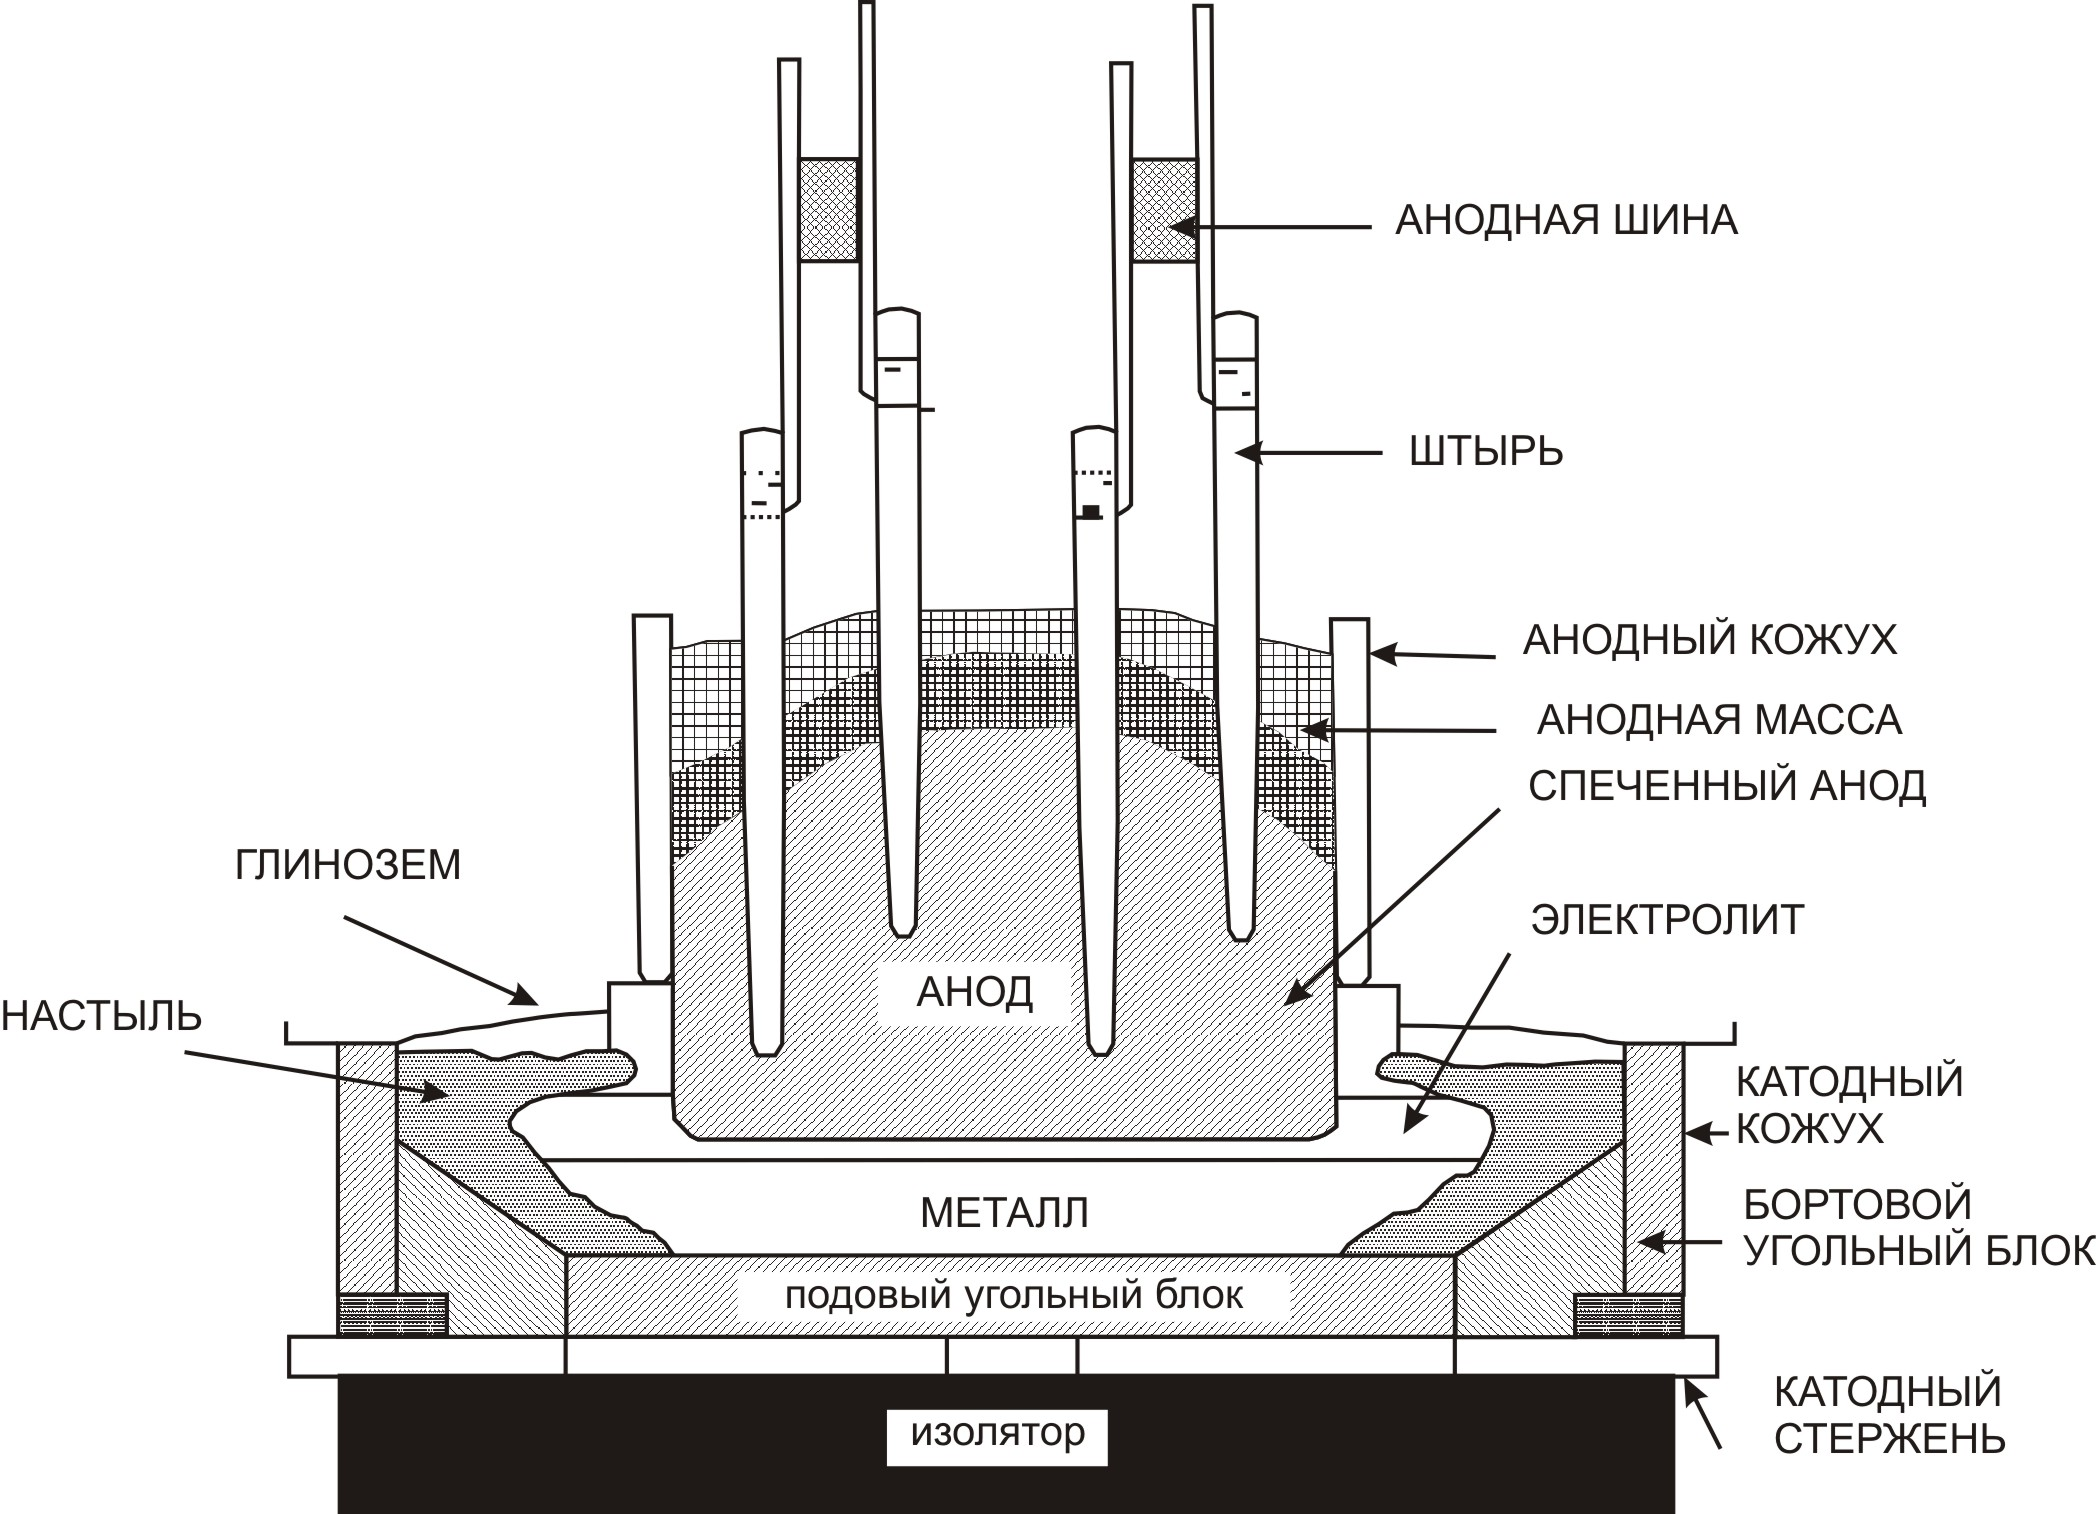
\includegraphics[width=0.8\linewidth]{Electrolizer.jpg}
\caption[]{}
\label{fig:elec}
Поперечный разрез алюминиевого электролизера с самообжигающимся анодом.
\end{figure}

Работу, которую совершает ток при прохождении через ванну, можно вычислить по формуле
\begin{equation}
 A=U \cdot I \cdot t,
\end{equation}
где U - напряжение на электролизере, I - сила тока, t - время (см. \cite{litlink:derkach}).

Теоретическое количество алюминия, которое должно получиться при электролизе, вычисляется по закону Фарадея
\begin{equation}\label{eq:faradey}
M=F \cdot I \cdot t.
\end{equation}

При этом количество реального произведенного металла всегда несколько меньше теоретического значения и вычисляется по формуле 
\begin{equation}\label{eq:real}
P=\eta \cdot F \cdot I \cdot t,
\end{equation}
где $\eta$ - выход по току, F - константа Фарадея (см. \cite{litlink:derkach}).

Для оценки эффективности производства необходимо связать количество полученного алюминия с затраченной энергией(удельный расход энергии)
\begin{equation}
W=\frac{A}{P}=\frac{U}{F \cdot \eta}.
\end{equation}
Обычно это величина колеблется от 12,5 до 18,0 кВт$\cdot$ч/кг. 

Из формул (\ref{eq:faradey}) и (\ref{eq:real}) следует, что
\begin{equation*}
\eta=\frac{P}{M},
\end{equation*}
где $\eta$ выход по току (безразмерный управляющий параметр).

На практике часто используют величину процентного выхода по току
\begin{equation}
\eta=\frac{100 \cdot P}{M}.
\end{equation}

Выход по току зависит от большого числа параметров: температуры, межполюсного расстояния (МПР), плотности тока, состава электролита, криолитового отношения (КО), конструкции, геометрии электролизеров, электромагнитных сил.

Перечислим основные физико-химические процессы проходящие в электролизной ванне \cite{litlink:kalmykov}, которые активно влияют друг на друга:
\begin{itemize}
\item гидродинамические процессы,
\item электромагнитные процессы,
\item химические процессы,
\item тепловые процессы
\end{itemize}

Гидродинамические процессы определяют циркуляцию вещества в расплаве электролита и в расплаве металла. Поскольку сырье в электролизер подается точечно, то распределение скоростей в электролите отвечает за перенос сырья в рабочем пространстве ванны. Неравномерное распределение загруженного в ванну глинозема ведет к потери выхода алюминия по току \cite{litink:AE}.

Магнитногидродинамические процессы, возникающие во время прохождения тока через электролизер, сильно влияют на МГД (Магнитногидродинамическую) стабильность ванны. 

Температура алюминия и подины также серьезно влияют на процесс производства, при снижении температуры расплава возможно образование коржей, которые уменьшают рабочую поверхность подины. В свою очередь слишком высокая температура приводит к расплавлению защитного слоя на боковых стенках ванны в зоне раздела металла.

Самым общим показателем эффективности управления процессом получения алюминия является себестоимость производства алюминия. Однако этот критерий зависит от большого числа параметров никак не связанных с самим процессом электролиза. Поэтому вводятся другие параметры приближенные к технологическому процессу. Это расход электроэнергии на тонну получаемого металла, удельный расход углерода и удельный расход фторидов. Эти управляющие параметры зависят друг от друга, однако их соотношения могут меняться в зависимости от специфики конкретного производства.

В ВАМИ (Всероссийский Алюминиево-магниевый Институт) было получено эмпирическое уравнение для расчета практического выхода по току \cite{litlink:VAMI}
\begin{equation} \label{eq1}
\eta=(1-2567 \cdot \frac{S^{0,21}_{anod}}{i^{0.58}_a \cdot L_{ACD} \cdot e^{\frac{12940}{T_e}}}) \cdot 100,
\end{equation}
где $i_a$ - анодная плотность тока, $S_{anod}$ - площадь анода, $L_{ACD}$ - МПР, $T_e$ - температура электролита.

В работе \cite{litlink:korobov} предложено следущее эмпирическое уравнение для расчета практического выхода алюминия:
\begin{equation} \label{eq:p}
P= \frac{wT-920}{0.336 \cdot \eta \cdot b}[0.112+\frac {1.12}{\delta \cdot (h+30)}+0.056 \cdot K],
\end{equation}
где T - температура электролита, $\eta$ - выход по току, b - выход углерода из анодной массы с учетом механических потерь, $\delta$ - анодная плотность тока, h - уровень жидкой массы, K - коэффициент тепловой нагрузки.

Формула Лилибуена \cite{litlink:Lillebuen} позволяет связать скорость потери алюминия и скорость на разделе веществ
\begin{equation}\label{eq:lilibuen}
R_{al} = 0,024 \cdot D_{al} \cdot l^{-0,17} \cdot V^{0,83} \cdot K \cdot \eta^{-0,5} \cdot \rho^{0,5}
\end{equation}
$R_{al}$ - скорость потери алюминия, $D_{al}$ - коэффициент диффузии алюминия в электролит, l - межполюсное расстояние, V - скорость на поверхности раздела электролит-металл, K - эмпирическая константа.

Также была получена формула для расчета снижения выхода по току в зависимости от деформации границы раздела \cite{litlink:derkach2}
\begin{equation} \label{eq2}
\Delta \eta = (1- \eta_0) \cdot \frac{l}{S} \cdot \int\limits_Z \frac{dxdy}{H(x,y)}
\end{equation}
$\Delta \eta$ - изменение выхода по току, l - значение МПР, $\eta_0$ - значение выхода по току при плоской поверхности раздела, S - площадь  поверхности раздела, $H(x,y)$ - высота металла.

Однако практическая реализация формулы (\ref{eq2}) зависит от точности определения функции, а также формы и площади границы раздела металл-электролит, если эти значения определены грубо, то погрешность формулы будет высока.

Таким образом в настоящее время судить о выходе по току в конкретной алюминиевой ванне можно ванне можно по формулам (\ref{eq1})-(\ref{eq2}). Однако в формулы (\ref{eq1})-(\ref{eq:lilibuen}) входят эмпирическими константы. Заметим, что в АСУТП на линии производства Красноярского завода внедрена формула (\ref{eq1}). Ясно, что наиболее точные значения должна давать формула (\ref{eq2}), но при условии, что поверхность раздела сред металл-электролит известна с высокой точностью.

\begin{figure}[H]
\centering
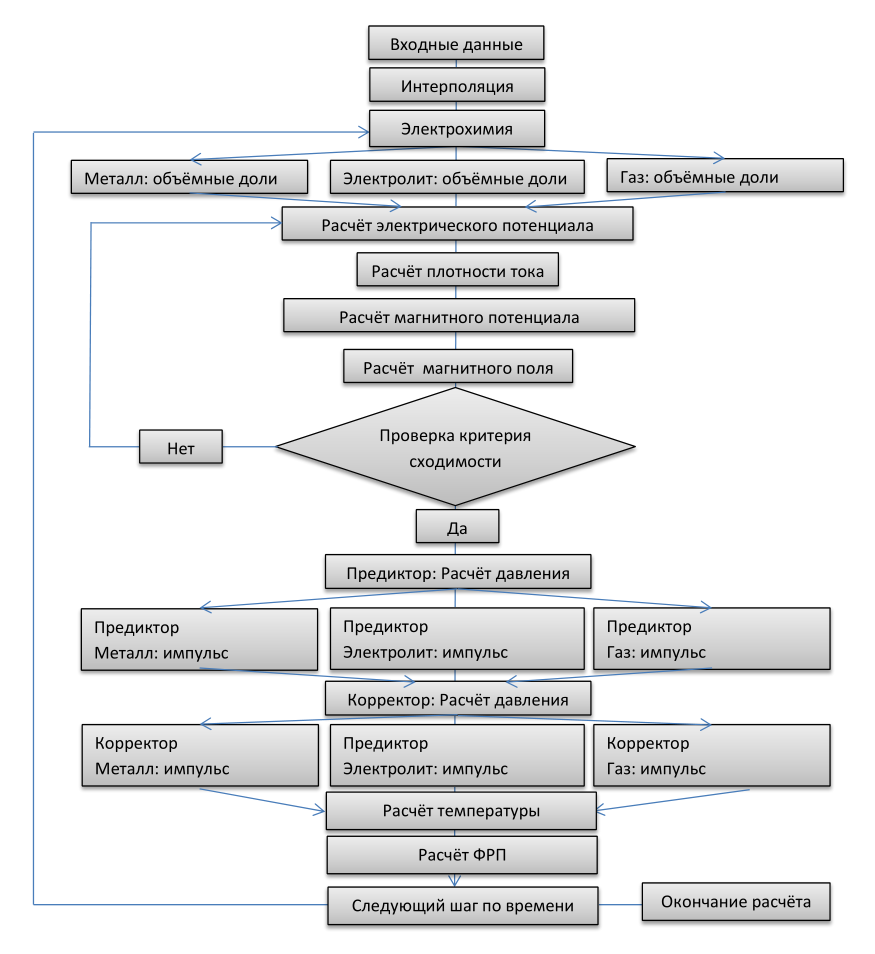
\includegraphics[width=0.8\linewidth]{scheme.png}
\caption[]{}
\label{fig:ASUTPscheme}
Схема работы АСУТП.
\end{figure}

В настоящей работе проводится математическое моделирование выхода по току конкретной алюминиевой ванны, физико-химические процессы в которой рассчитываются с помощью математической модели промышленной электролизной ванны подробно описанной в работе \cite{litlink:kalmykov}.

\section{Исследование способов вычисления выхода по току}

\subsection{Вычисление выхода по току по эмпирической формуле}
%\addcontentsline{toc}{section}{Вычисление выхода по току по эмпирической формуле}
Требуется провести вычисления выхода потоку при помощи эмпирической формулы (\ref{eq1}).

Приведем конкретные значения параметров в формуле (\ref{eq1}):
\begin{itemize}
\item Сила тока $I=250 $кА,
\item Длинна ванны $a=9.4$м,
\item Ширина ванны $b=3.4$м,
\item МПР 23.1 см,
\item $970 C^{\circ}$.
\end{itemize}
Таким образом плотность тока рассчитывается по формуле
\begin{equation}
i_a = \frac{I}{a \cdot b}
\end{equation}
Тогда выход потоку по формуле (\ref{eq1})
\begin{equation}
\eta=(1-2567 \cdot \frac{15.876^{0,21}}{0.688^{0.58}_a \cdot 0.231 \cdot e^{\frac{12940}{970}}}) \cdot 100 \approx 96.0318.
\end{equation}

Ниже на рисунках \ref{fig:SPlot}-\ref{fig:TPlot} демонстрируется вычисленная по формуле (\ref{eq1}) зависимость выхода по току от:
\begin{enumerate}
\item площади ванны при постоянной плотности тока (рис. \ref{fig:SPlot}),
\item площади ванны при постоянной силе тока (рис. \ref{fig:SaPlot}),
\item силы тока (рис. \ref{fig:IPlot}),
\item плотности тока (рис. \ref{fig:iPlot}),
\item МПР (рис. \ref{fig:LPlot}),
\item температуры расплава(рис. \ref{fig:TPlot}).
\end{enumerate}
\begin{figure}[H]
\centering
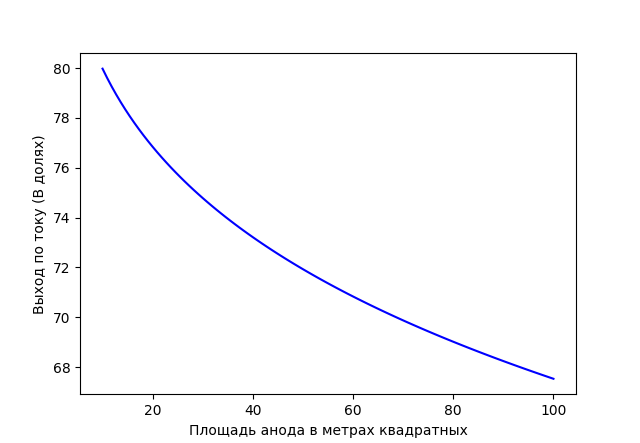
\includegraphics[width=0.8\linewidth]{S.png}
\caption{}
\label{fig:SPlot}
Зависимость выхода по току от площади ванны при постоянной плотности тока
\end{figure}

\begin{figure}[H]
\centering
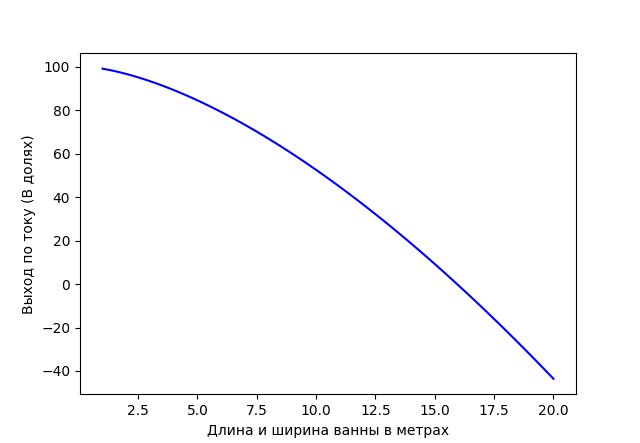
\includegraphics[width=0.8\linewidth]{Sa.png}
\caption{}
\label{fig:SaPlot}
Зависимость выхода по току от площади ванны при постоянной силе тока
\end{figure}

\begin{figure}[H]
\centering
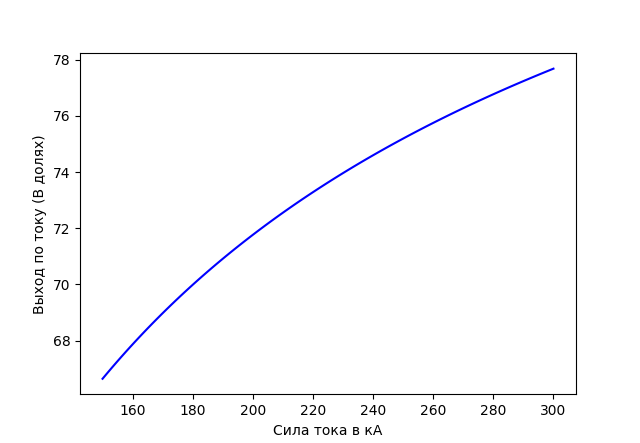
\includegraphics[width=0.8\linewidth]{I.png}
\caption{}
Зависимость выхода по току от силы тока
\label{fig:IPlot}
\end{figure}

\begin{figure}[H]
\centering
\includegraphics[width=0.8\linewidth]{i.png}
\caption{}
\label{fig:iPlot}
Зависимость выхода по току от плотности тока
\end{figure}

\begin{figure}[H]
\centering
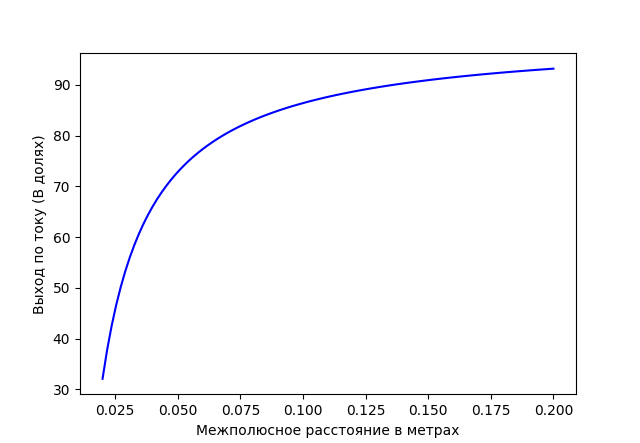
\includegraphics[width=0.8\linewidth]{L.png}
\caption{}
\label{fig:LPlot}
Зависимость выхода по току от МПР
\end{figure}

\begin{figure}[H]
\centering
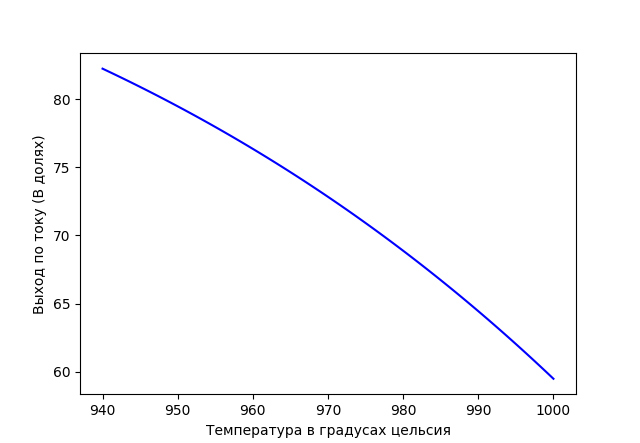
\includegraphics[width=0.8\linewidth]{T.png}
\caption{}
\label{fig:TPlot}
Зависимость выхода по току от температуры
\end{figure}

Таким образом из рисунков \ref{eq1} - \ref{eq2} видно, что управляющий параметр сильно зависит от размеров ванны и размера анода, от силы и плотности тока, от температуры и МПР. Заметим, что наиболее сложно из всех перечисленных величин замерить значение МПР. Замеры МПР на практике осуществляется путем анализа расплава металлического стержня опущенного в рабочее пространство ванны. Даже если такой эксперементальный замер производится в нескольких точках ванны, представление о минимальном МПР получается весьма приближенным, что как видно из рисунка \ref{fig:LPlot} может сильно повлиять на величину управляющего параметра выхода по току.

\subsection{Расчёт потери по току по теоретической формуле.}\label{sec:teor}

Предлагается два варианта численных методов для вычисления поверхностного интеграла в формуле (\ref{eq1}).

Используем квадратурную формулу трапеций для вычисления интеграла
\begin{equation} \label{eq:int}
I = \iint\limits_Z f(x,y) dS.
\end{equation}

Величина I по методу центральных прямоугольников на равномерной сетке по каждому направлению с шагами $h_x$ и $h_y$ с числом узлов (n+1) и (k+1) соответственно вычисляется по формуле
\begin{align}\label{eq:squaremethod}
I_{nk} = \sum\limits_{j=0}^{k} \sum\limits_{i=0}^{n} f(\frac{x_i+x_{i+1}}{2},\frac{y_j+y_{j+1}}{2}) \cdot h_x \cdot h_y
\end{align}
Ниже демонстрируется применение формулы (\ref{eq:int}) для поверхности Z(x,y) заданной в явном виде в аналитической форме. Тогда известно \cite{ litlink:Kudryavcev}, что 
\begin{align}
\iint\limits_Z f(x,y) dS = \label{eq:analit}
\iint\limits f(x,y) \cdot \sqrt{(1+(\frac{dZ(x,y)}{dx})^2+ (\frac{dZ(x,y)}{dy})^2)}dxdy,
\end{align}

\subsubsection*{Пример 1}\label{ex1m}
\addcontentsline{toc}{subsubsection}{Пример 1} 
Пусть поверхность раздела сред металл-электролит задана уравнением
\begin{equation} \label{eq:surf1}
Z(x,y) = 0.44 + 0.003x + 0.004y.
\end{equation}
Поверхность Z, определенная формулой (\ref{eq:surf1}), изображена на рисунке \ref{fig:H1Surf}. Площадь анодов для этой ванны возьмем $40$.

Будем считать, что эта поверхность является разделом металл - электролит электролизной ванны размеры которой зафиксированны выше. Тогда величина l соответствует минимальному расстоянию от поверхности Z до подошвы анода, $l=1 cm$.

\begin{figure}[H]
\centering
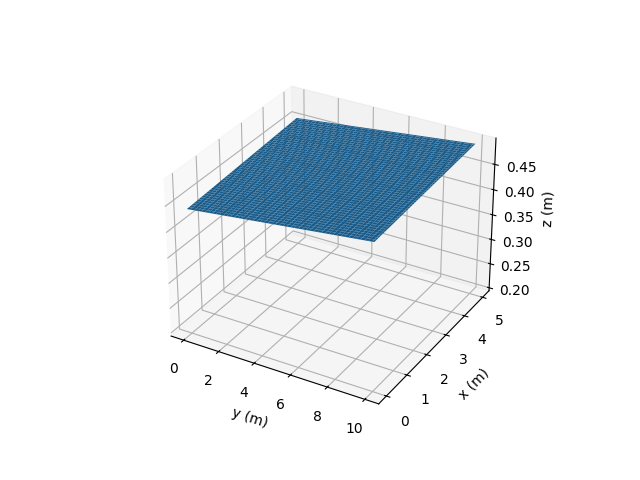
\includegraphics[width=0.8\linewidth]{First_surface.png}
\caption{}
\label{fig:H1Surf}
Разделяющая поверхность
\end{figure}

Проведем вычисления потери выхода по току по формуле (\ref{eq2}). При этом  интеграл по поверхности будем вычислять по формуле (\ref{eq:analit}).


Аналитическое вычисление по формуле (\ref{eq:analit})
\begin{align} \label{eq:analit1:min}
\Delta \eta = 0,1 \cdot \frac{0.01}{40} \int\limits_0^{10} \int\limits_0^5 \frac{\sqrt{1+(0,003)^2+(0,004)^2}}{0.44 + 0.003x + 0.004y} dy dx = \notag \\
= \frac{0,1 \cdot 0.01\sqrt{1+(0,003)^2+(0,004)^2}}{40 \cdot 0,004} \cdot \notag \\
\cdot \int\limits_0^{10} ln(0.44 + 0.003x + 0.004y)|_0^5 dx = \notag \\
= \frac{0,1 \cdot 0.01\sqrt{1+(0,003)^2+(0,004)^2}}{40 \cdot 0,004} \cdot \notag \\
\cdot \bigl(\int\limits_0^{10} ln(0.44 + 0.003x + 0.02)dx - \int\limits_0^{10} ln(0.44 + 0.003x)dx \bigr) = \notag \\
= \frac{-0,1 \cdot 0.01\sqrt{1+(0,003)^2+(0,004)^2}}{40 \cdot 0,004 \cdot 0.003} \cdot \notag \\
\cdot \bigl(((0,46+0,003x) \cdot ln(0,46+0,003x) - (0,46+0,003x))|_0^{10} - \notag \\
- ((0,46+0,003x) \cdot ln(0,346+0,003x) - (0,346+0,003x))|_0^{10}\bigr) = \notag \\
= \frac{-0,1 \cdot 0.01\sqrt{1+(0,003)^2+(0,004)^2}}{40 \cdot 0,004 \cdot 0.003} \cdot \notag \\
\cdot \bigl(0,47 ln(0.47)-0,44ln(0,44)-0,03- \notag \\
- (0,49ln(0,49)-0,46ln(0,46)-0,03)\bigr) = \notag \\
= 0.002689559
\end{align}
Вычисления по квадратурной формуле (\ref{eq:squaremethod}), n=k=100
\begin{align}\label{eq:sq1min10}
\Delta \eta = 0,1 \cdot \frac{0.01}{50.000625} \int\limits_0^{10} \int\limits_0^5 \frac{\sqrt{1+(0,003)^2+(0,004)^2}}{0.44 + 0.003x + 0.004y} dy dx \approx \notag \\ \approx 0.0026910167819670706
\end{align}
Вычисления по квадратурной формуле (\ref{eq:squaremethod}), n=k=50
\begin{align}\label{eq:sq1min5}
\Delta \eta = 0,1 \cdot \frac{0.01}{50.000625} \int\limits_0^{10} \int\limits_0^5 \frac{\sqrt{1+(0,003)^2+(0,004)^2}}{0.44 + 0.003x + 0.004y} dy dx \approx \notag \\ \approx 0.002692510716716919
\end{align}

Проведем аналогичные вычисления для другого значения l, пусть $l=0.06$ (соответствует точке на поверхности Z(x,y) в центре).

Аналитическое решение по формуле (\ref{eq:analit})
\begin{align} \label{eq:analit1:med}
\Delta \eta = 0,1 \cdot \frac{0.01}{40} \int\limits_0^{10} \int\limits_0^5 \frac{\sqrt{1+(0,003)^2+(0,004)^2}}{0.44 + 0.003x + 0.004y} dy dx = \notag \\
= \frac{0,1 \cdot 0.01\sqrt{1+(0,003)^2+(0,004)^2}}{40 \cdot 0,004} \cdot \notag \\
\cdot \int\limits_0^{10} ln(0.44 + 0.003x + 0.004y)|_0^5 dx = \notag \\
= \frac{0,1 \cdot 0.01\sqrt{1+(0,003)^2+(0,004)^2}}{40 \cdot 0,004} \cdot \notag \\
\cdot \bigl(\int\limits_0^{10} ln(0.44 + 0.003x + 0.02)dx - \int\limits_0^{10} ln(0.44 + 0.003x)dx \bigr) = \notag \\
= \frac{-0,1 \cdot 0.01\sqrt{1+(0,003)^2+(0,004)^2}}{40 \cdot 0,004 \cdot 0.003} \cdot \notag \\
\cdot \bigl(((0,46+0,003x) \cdot ln(0,46+0,003x) - (0,46+0,003x))|_0^{10} - \notag \\
- ((0,46+0,003x) \cdot ln(0,346+0,003x) - (0,346+0,003x))|_0^{10}\bigr) = \notag \\
= \frac{-0,1 \cdot 0.01\sqrt{1+(0,003)^2+(0,004)^2}}{40 \cdot 0,004 \cdot 0.003} \cdot \notag \\
\cdot \bigl(0,47 ln(0.47)-0,44ln(0,44)-0,03- \notag \\
- (0,49ln(0,49)-0,46ln(0,46)-0,03)\bigr) = \notag \\
= 0.016137327
\end{align}
Вычисления по квадратурной формуле (\ref{eq:squaremethod}), n=k=100
\begin{align}\label{eq:sq1med10}
0,1 \cdot \frac{0.06}{40} \int\limits_0^{10} \int\limits_0^5 \frac{\sqrt{1+(0,003)^2+(0,004)^2}}{0.44 + 0.003x + 0.004y} dy dx \approx \notag \\ \approx 0.016146100691802452
\end{align}
Вычисления по квадратурной формуле (\ref{eq:squaremethod}), n=k=50
\begin{align}\label{eq:sq1med5}
0,1 \cdot \frac{0.06}{40} \int\limits_0^{10} \int\limits_0^5 \frac{\sqrt{1+(0,003)^2+(0,004)^2}}{0.44 + 0.003x + 0.004y} dy dx \approx \notag \\ \approx 0.01615506430030167
\end{align}

Проведем вычисления для $l=0.11$ (соответствует точке на поверхности Z(x,y) в правом верхнем углу).

Аналитическое решение по формуле (\ref{eq:analit})
\begin{align}\label{eq:analit1:max}
\Delta \eta = 0,1 \cdot \frac{0.11}{40} \int\limits_0^{10} \int\limits_0^5 \frac{\sqrt{1+(0,003)^2+(0,004)^2}}{0.44 + 0.003x + 0.004y} dy dx = \notag \\
= \frac{0,1 \cdot 0.01\sqrt{1+(0,003)^2+(0,004)^2}}{40 \cdot 0,004} \cdot \notag \\
\cdot \int\limits_0^{10} ln(0.44 + 0.003x + 0.004y)|_0^5 dx = \notag \\
= \frac{0,1 \cdot 0.01\sqrt{1+(0,003)^2+(0,004)^2}}{40 \cdot 0,004} \cdot \notag \\
\cdot \bigl(\int\limits_0^{10} ln(0.44 + 0.003x + 0.02)dx - \int\limits_0^{10} ln(0.44 + 0.003x)dx \bigr) = \notag \\
= \frac{-0,1 \cdot 0.01\sqrt{1+(0,003)^2+(0,004)^2}}{40 \cdot 0,004 \cdot 0.003} \cdot \notag \\
\cdot \bigl(((0,46+0,003x) \cdot ln(0,46+0,003x) - (0,46+0,003x))|_0^{10} - \notag \\
- ((0,46+0,003x) \cdot ln(0,346+0,003x) - (0,346+0,003x))|_0^{10}\bigr) = \notag \\
= \frac{-0,1 \cdot 0.01\sqrt{1+(0,003)^2+(0,004)^2}}{40 \cdot 0,004 \cdot 0.003} \cdot \notag \\
\cdot \bigl(0,47 ln(0.47)-0,44ln(0,44)-0,03- \notag \\
- (0,49ln(0,49)-0,46ln(0,46)-0,03)\bigr) = \notag \\
= 0.02958512
\end{align}
Вычисления по квадратурной формуле (\ref{eq:squaremethod}), n=k=100
\begin{align}\label{eq:sq1max10}
\Delta \eta = (1- \eta_0) \cdot \frac{l}{S} \cdot \iint\limits_Z \frac{\sqrt{(1+(\frac{dz}{dx})^2+ (\frac{dz}{dy})^2)}}{H(x,y)}dxdy = \notag \\
= 0,1 \cdot \frac{0.11}{40} \int\limits_0^{10} \int\limits_0^5 \frac{\sqrt{1+(0,003)^2+(0,004)^2}}{0.44 + 0.003x + 0.004y} dy dx \approx \notag \\
\approx 0.02960118460163804
\end{align}
Вычисления по квадратурной формуле (\ref{eq:squaremethod}), n=k=50
\begin{align}\label{eq:sq1max5}
\Delta \eta = (1- \eta_0) \cdot \frac{l}{S} \cdot \iint\limits_Z \frac{\sqrt{(1+(\frac{dz}{dx})^2+ (\frac{dz}{dy})^2)}}{H(x,y)}dxdy = \notag \\
= 0,1 \cdot \frac{0.2}{40} \int\limits_0^{10} \int\limits_0^5 \frac{\sqrt{1+(0,003)^2+(0,004)^2}}{0.44 + 0.003x + 0.004y} dy dx \approx \notag \\ 
\approx 0.029617617883886373
\end{align}

Анализ результатов проведенных расчетов показывает, что величина l сильно влияет на значение параметра потери выхода по току. При этом расчеты вариантов b наиболее близки к соответствующим значениям, вычисленным аналитически. 

\subsubsection*{Пример 2}\label{ex2m}
\addcontentsline{toc}{subsubsection}{Пример 2}
Пусть поверхность раздела сред металл-электролит задана уравнением
\begin{equation}\label{eq:surf2}
z(x,y)=0,44+0,05 \cdot sin(x) \cdot cos(y)
\end{equation}

Поверхность Z, определенная формулой (\ref{eq:surf2}), изображена на рисунке \ref{fig:H2Surf}. Площадь андов для этой ванны будем считать $40 m^2$.

Будем считать, что эта поверхность является разделом металл - электролит электролизной ванны размеры которой зафиксированны выше. Тогда величина l соответствует минимальному расстоянию от поверхности Z до подошвы анода, $l=1 cm$.

\begin{figure}[H]
\centering
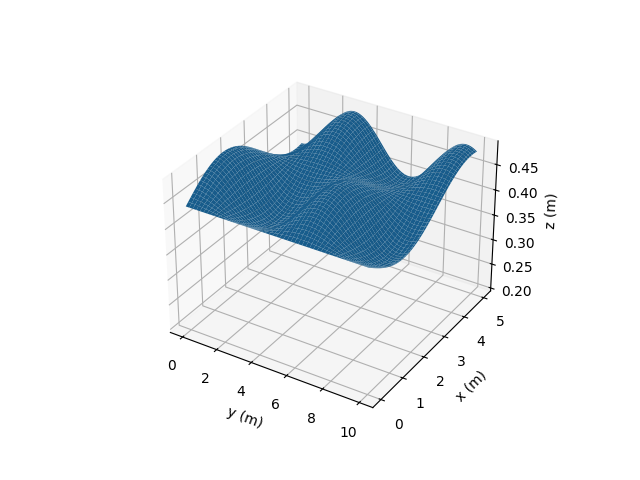
\includegraphics[width=0.8\linewidth]{Second_surface.png}
\caption{}
\label{fig:H2Surf}
Разделяющая поверхность
\end{figure}


Вычисления по квадратурной формуле (\ref{eq:squaremethod}), n=k=100
\begin{align}\label{eq:sq2min10}
\Delta \eta = 0,1 \cdot \frac{0,01}{40} \cdot \notag \\
\cdot \int\limits_0^{10} \int\limits_0^5 \frac{\sqrt{1+0.05cos(x)cos(y)-0.05sin(x)sin(y)}}{0.44 + 0.05sin(x)cos(y)} dy dx \approx \notag \\ \approx 0.0028705181744004275
\end{align}
Вычисления по квадратурной формуле (\ref{eq:squaremethod}), n=k=50
\begin{align}\label{eq:sq2min5}
\Delta \eta = 0,1 \cdot \frac{0,05}{40}  \cdot \notag \\
\cdot \int\limits_0^{10} \int\limits_0^5 \frac{\sqrt{1+0.05cos(x)cos(y)-0.05sin(x)sin(y)}}{0.44 + 0.05 \cdot sin(x) \cdot cos(y)} dy dx \approx \notag \\ \approx 0.002870213860349491
\end{align}

Проведем аналогичные вычисления для другого значения l, пусть $l=0.06$ (соответствует точке на поверхности Z(x,y) в точках $sin(x)=0$ или $cos(y)=0$).

Вычисления по квадратурной формуле (\ref{eq:squaremethod}), n=k=100
\begin{align}\label{eq:sq2med10}
\Delta \eta = 0,1 \cdot \frac{0,06}{40} \cdot \notag \\
\cdot \int\limits_0^{10} \int\limits_0^5 \frac{\sqrt{1+0.05cos(x)cos(y)-0.05 sin(x)sin(y)}}{0.44 + 0.05 \cdot sin(x) \cdot cos(y)} dy dx \approx \notag \\ \approx 0.01722310904640258
\end{align}
Вычисления по квадратурной формуле (\ref{eq:squaremethod}), n=k=50
\begin{align}\label{eq:sq2med5}
\Delta \eta = 0,1 \cdot \frac{0,06}{40} \cdot \notag \\
\cdot \int\limits_0^{10} \int\limits_0^5 \frac{\sqrt{1+0.05cos(x)cos(y)-0.05 sin(x)sin(y)}}{0.44 + 0.05 \cdot sin(x) \cdot cos(y)} dy dx \approx \notag \\ \approx 0.017221283162096944
\end{align}

Проведем вычисления для $l=0.11$ (соответствует точке на поверхности Z(x,y) на "пике").

Аналитическое решение по формуле (\ref{eq:analit})

Вычисления по квадратурной формуле (\ref{eq:squaremethod}), n=k=100
\begin{align}\label{eq:sq2max10}
\Delta \eta = 0,1 \cdot \frac{0.11}{40} \cdot \notag \\
\cdot \int\limits_0^{10} \int\limits_0^5 \frac{\sqrt{1+0.05cos(x)cos(y)-0.05 sin(x)sin(y)}}{0.44 + 0.05 \cdot sin(x) \cdot cos(y)} dy dx \approx \notag \\ \approx 0.0315756999184048
\end{align}
Вычисления по квадратурной формуле (\ref{eq:squaremethod}), n=k=50
\begin{align}\label{eq:sq2max5}
\Delta \eta = 0,1 \cdot \frac{0.11}{40} \cdot \notag \\
\cdot \int\limits_0^{10} \int\limits_0^5 \frac{\sqrt{1+0.05cos(x)cos(y)-0.05 sin(x)sin(y)}}{0.44 + 0.05 \cdot sin(x) \cdot cos(y)} dy dx \approx \notag \\ \approx 0.03157235246384434
\end{align}

\subsection{Модифицированная теоретическая формула вычисления потери по току.}\label{sec:mod}

Для расчета потери выхода по току по теоретической формуле (\ref{eq2}) используется параметр выхода по току при плоской границе раздела сред $\eta_0$. Поскольку поверхность раздела сред Z меняется во времени, то ее площадь S также меняется во времени. В свою очередь величина l может быть разной в зависимости от точке в которой проводится измерение. Как показано в работе \cite{litlink:kalmykov} граница раздела  сред электролит-газ, соответствующая зоне обратного окисления металла, также сильно влияет на величину l, а значит на величину потерь выхода по току.

В формуле (\ref{eq2}) значения параметров l и S являются константами, которые определяются опытным путем с большой погрешностью. Поэтому в настоящей работе предлагается следущая модификация формулы (\ref{eq2}).
\begin{equation} \label{eq:modeq2}
\Delta \eta = (1- \eta_0) \cdot \frac{1}{S} \cdot \iint\limits_Z \frac{l(x,y)}{H(x,y)}dS.
\end{equation}

Ниже приводится вычисления тремя способами значения потери по току для различных поверхностей Z(x,y).

\subsubsection*{Пример 1}
\addcontentsline{toc}{subsubsection}{Пример 1}

Поверхность Z, определенная формулой (\ref{eq:surf1}), изображена на рисунке \ref{fig:H1Surf}. Площадь анодов равняется $40$ также, как и выше.

Вычисления по квадратурной формуле (\ref{eq:squaremethod}), n=k=100
\begin{align}
\Delta \eta = 0,1 \cdot \frac{1}{40} \int\limits_0^{10} \int\limits_0^5 (0.06 - 0.44 + 0.003x + 0.004y) \cdot \notag \\
\cdot \sqrt{1+(0,003)^2+(0,004)^2}/ \notag \\ 
/(0.44 + 0.003x + 0.004y) dy dx \approx \notag \\ \approx 0.009549276608118927
\end{align}
Вычисления по квадратурной формуле (\ref{eq:squaremethod}), n=k=50
\begin{align}
\Delta \eta = 0,1 \cdot \frac{1}{40} \int\limits_0^{10} \int\limits_0^5 (0.06 - 0.44 + 0.003x + 0.004y) \cdot \notag \\
\cdot \sqrt{1+(0,003)^2+(0,004)^2}/ \notag \\ 
/(0.44 + 0.003x + 0.004y) dy dx \approx \notag \\ \approx 0.00962397334561231
\end{align}

\subsubsection*{Пример 2}
\addcontentsline{toc}{subsubsection}{Пример 2}

Поверхность Z, определенная формулой (\ref{eq:surf1}), изображена на рисунке \ref{fig:H1Surf}. Площадь анодов равняется $40$ также, как и выше.

Вычисления по квадратурной формуле (\ref{eq:squaremethod}), n=k=100
\begin{align}
\Delta \eta = 0,1 \cdot \frac{1}{40} \cdot \notag \\
\cdot \int\limits_0^{10} \int\limits_0^5 (0,06 - 0,05sin(x)cos(y)) \cdot \notag \\
\cdot \sqrt{1+0.05cos(x)cos(y)-0.05sin(x)sin(y)}/ \notag \\
/(0.44 + 0.05sin(x)cos(y)) dy dx \approx \notag \\ \approx 0.018253636056426627
\end{align}
Вычисления по квадратурной формуле (\ref{eq:squaremethod}), n=k=4
\begin{align}
\Delta \eta = 0,1 \cdot \frac{1}{40} \cdot \notag \\
\cdot \int\limits_0^{10} \int\limits_0^5 (0,06 - 0,05sin(x)cos(y)) \cdot \notag \\
\cdot \sqrt{1+0.05cos(x)cos(y)-0.05sin(x)sin(y)}/ \notag \\
/(0.44 + 0.05sin(x)cos(y)) dy dx \approx \notag \\ \approx 0.018252353331560892
\end{align}

Модифицированная формула дает существенно отличный результат от полученного в формуле \ref{eq2}.

\section{Вычисление потери выхода по току для поверхности границы раздела сред металл - электролит произвольного вида.}
\subsection{Вывод формулы вычисления поверхности при помощи метода триангуляции}

В пунктах \ref{sec:teor} и \ref{sec:mod} поверхность раздела задавалась аналитически. Однако в вычислительном комплексе математического моделирования процесса промышленного электролиза алюминия границы раздела сред металл-электролит и газ-электролит получаются в результате численного расчета и задаются таблично. Поэтому интегралы в формулах (\ref{eq1}) и (\ref{eq:modeq2}) эффективно вычислять методом триангуляции.

В работах \cite{litlink:scvortsov} и \cite{litlink:shirok} подробно описаны способы построения триангуляции для сложных поверхностей с неравномерно заданными на плоскости точками. В настоящей работе предлагается алгоритм вычисления поверхностного интеграла для границы раздела металл-электролит произвольной конфигурации, адаптированного к равномерной сетке по каждому пространственному  направлению. При этом именно эта равномерная сетка используется в вычислениях комплекса реализующем математическую модель электролиза алюминия в промышленной ванне (см. \cite{litlink:kalmykov}). Однако эти методы сложны в реализации.

Выпишем формулы триангуляции для простой прямоугольной поверхности с разбиением на элементарные треугольники.

На плоскости водится равномерная сетка размером $N$ на $M$ с шагами $x_h$, $h_y$ и узлами $P_{i,j}$. В узлах этой сетки таблично задается подынтегральная функция $f_{i,j}$. Плоскость разбивается на $2 \cdot N \cdot M$ прямоугольных треугольников как показано на рисунке \ref{fig:grid}.

\begin{figure}[H]
\centering
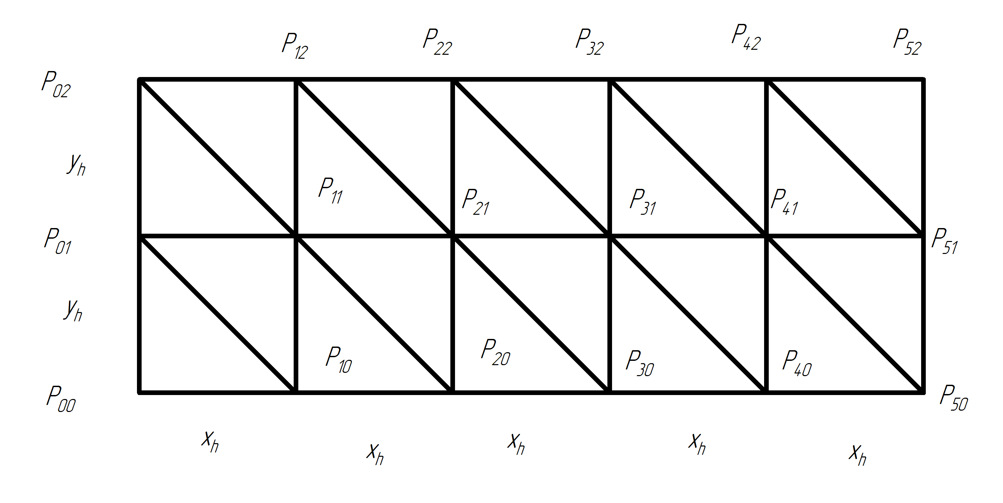
\includegraphics[width=0.8\linewidth]{Сетка.png}
\caption{}
\label{fig:grid}
Разбиение рассчетной области на треугольники.
\end{figure}

Каждый из этих треугольников соответствует поверхностному треугольнику в поверхности Z, как показано на рисунке \ref{fig:triangle}.

\begin{figure}[H]
\centering
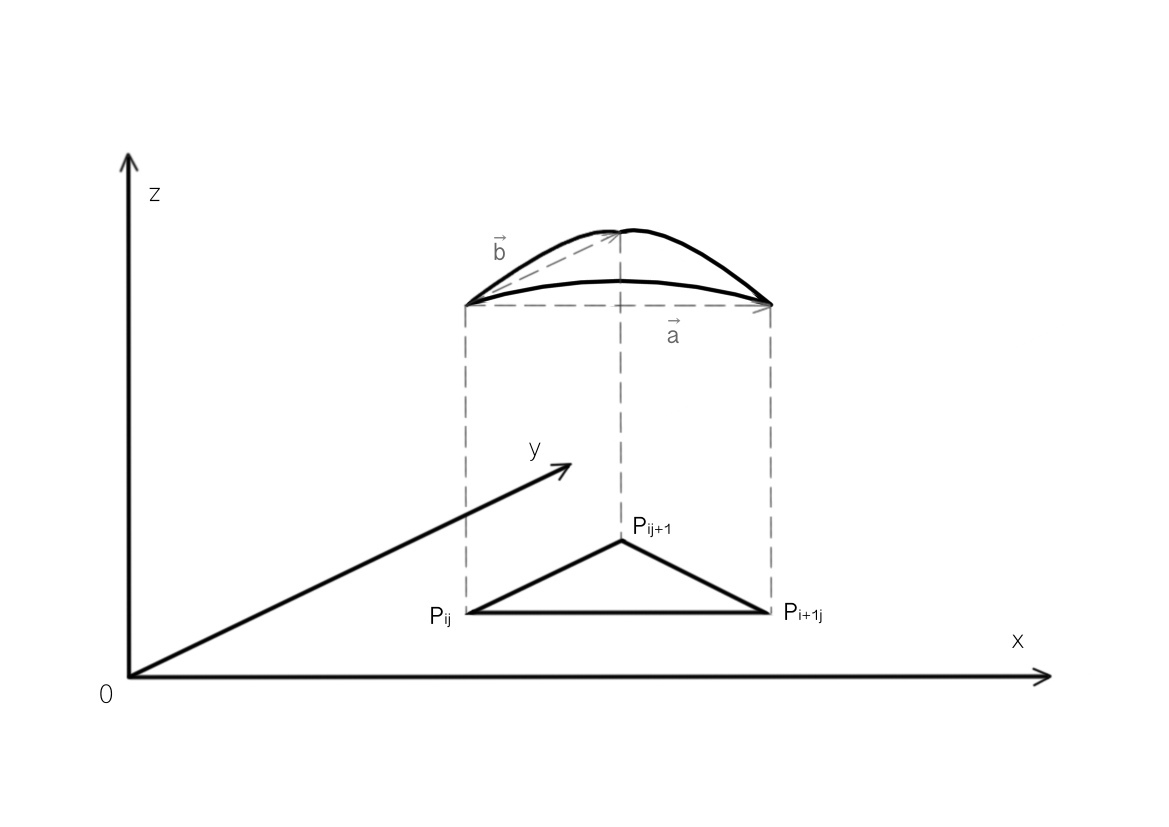
\includegraphics[width=0.8\linewidth]{Triangle.jpg}
\caption{}
\label{fig:triangle}
Проекция поверхности раздела на расчетную сетку.
\end{figure}

Площади поверхностных треугольников $P_{i,j}, P_{i,j+1}, P_{i+1,j}$ считается по формуле 

\begin{align}\label{eq:triangle_square}
S_{\triangle_{i,j}^1} = \frac{1}{2} \lvert [\overline{P_{i,j}P_{i,j+1}};\overline{P_{i,j}P_{i+1,j}}] \rvert = \lvert \frac{1}{2} 
\begin{vmatrix}
  I & J & K \\
  h_x & 0 & f_{i+1,j}-f_{i,j} \\
  0 & h_y & f_{i,j+1}-f_{i,j}
\end{vmatrix}
\rvert
= \notag \\
= \lvert I \cdot (-(f_{i+1,j}-f_{i,j}) \cdot h_y) - h_x \cdot (J \cdot (f_{i,j+1}-f_{i,j}) - h_y \cdot K) \rvert = \notag \\
= \lvert I \cdot h_y \cdot f_{i,j} -I \cdot h_y \cdot f_{i+1,j} - h_x \cdot J \cdot f_{i,j+1}+ h_x \cdot J \cdot f_{i,j} + h_x \cdot h_y \cdot K \rvert = \notag \\
= (h_y \cdot f_{i,j} - \cdot h_y \cdot f_{i+1,j})^2 + (h_x \cdot f_{i,j} - h_x \cdot f_{i,j+1})^2 + (h_x \cdot h_y)^2 \\
S_{\triangle_{i,j}^2} = \frac{1}{2} \lvert [\overline{P_{i+1,j+1}P_{i,j+1}};\overline{P_{i+1,j+1}P_{i+1,j}}] \rvert = \notag \\
= (h_y \cdot f_{i+1,j+1} - \cdot h_y \cdot f_{i+1,j})^2 + (h_x \cdot f_{i+1,j+1} - h_x \cdot f_{i,j+1})^2 + (h_x \cdot h_y)^2,
\end{align}
где I,J,K орты соответственно осей X,Y,Z.

Пронумеруем треугольники как показано на рисунке \ref{fig:triangle_numeration}.

\begin{figure}[H]
\centering
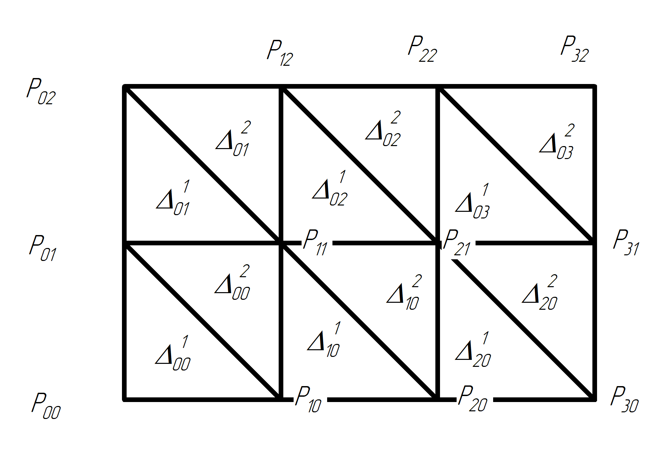
\includegraphics[width=0.8\linewidth]{triangle_numeration.png}
\caption{}
\label{fig:triangle_numeration}
Порядок нумерации введённых треугольников на расчётной сетке.
\end{figure}

Каждому $\triangle^n_{i,j}$ соответствует значение функции  $F^n_{i,j}$, получим значение для двумерного по аналогии с одномерным случаем:

\begin{enumerate}
\item Одномерный случай.

В одномерном случае рассматривается интеграл
\begin{align}
I= \int\limits_a^b f(x) dx.
\end{align}
Для его вычисления, область интегрирования (отрезок $[a,b]$) разбивается на элементарные отрезки $[x_i, x_{i+1}]$. Каждому элементарному отрезку соответствует значение функции $f_i$, тогда приближенное значение интеграла на этом отрезке $\widetilde{I}=(x_{i+1}-x_{i}) \cdot f_i$.

Построим интерполяционный полином Лагранжа на этом отрезке
\begin{align}
L(x) = \frac{x-x_{i+1}}{x_i-x_{i+1}} \cdot f_i+ \frac{x-x_i}{x_{i+1}-x_{i}} \cdot f_{i+1} = \notag \\
= \frac{1}{x_{i+1}-x_{i}} ((x-x_{i})\cdot f_{i+1}-(x-x_{i+1}) \cdot f_{i}).
\end{align}
Тогда,
\begin{align}
\widetilde{I} = \int\limits_{x_{i}}^{x_{i+1}} L(x) dx = \notag \\
= \frac{1}{x_{i+1}-x_{i}} (f_{i+1} \int\limits_{x_{i}}^{x_{i+1}} (x-x_{i}) dx - f_i \int\limits_{x_{i}}^{x_{i+1}} (x-x_{i+1}) dx) = \notag \\
= \frac{1}{x_{i+1}-x_{i}} (f_{i+1} \cdot (\frac{1}{2} (x_{i+1}^2 - x_{i}^2) -x_i x_{i+1}+x_{i}^2)) - \notag \\
- f(x_{i}) (\frac{1}{2} (x_{i+1}^2-x_{i}^2)-x_{i+1}^2+x_i x_{i+1})) = \notag \\
= \frac{1}{x_{i+1}-x_{i}} \cdot \notag \\
\cdot (f_{i+1} \cdot (\frac{1}{2} (x_{i+1}^2 + x_{i}^2) -x_i x_{i+1}) + f_i (\frac{1}{2}(x_{i+1}^2+x_{i}^2)-x_i x_{i+1})) = \notag \\
= \frac{1}{x_{i+1}-x_{i}} (f_{i+1}+ f_i) \cdot (\frac{1}{2} (x_{i+1}^2 + x_{i}^2) -x_i x_{i+1}) = \notag \\
= (x_{i+1}-x_{i}) \cdot \frac{1}{2}(f_i+f_{i+1})
\end{align}

Тогда f на элементарном отрезке.
\begin{align}
F_i = \frac{1}{2}(f_{i}+f_{i+1})
\end{align}

$F_i$ аппроксимирует значение функции со вторым порядком точности \cite{litlink:samarskiy} в середине отрезка.

Аналогично с одномерным случаем вычислим значение двумерного поверхностного интегала

\item Двумерный случай

Применим вышеописанный метод разбиения поверхности. Разобьём поверхность на элементарные фрагменты, как показано на рисунке 1. Каждому из которых поставим в соответствии треугольник ABC.

\begin{figure}[H]
\centering
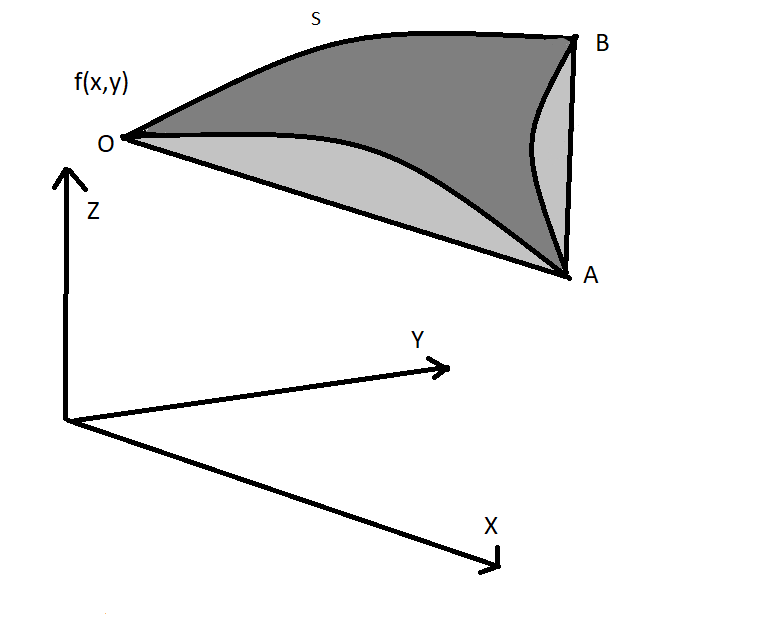
\includegraphics[width=0.8\linewidth]{triangleL.png}
\caption[]{}
\label{fig:L}
Фрагмент поверхности с соответствующим ему треугольником.
\end{figure}

\begin{figure}[H]
\centering
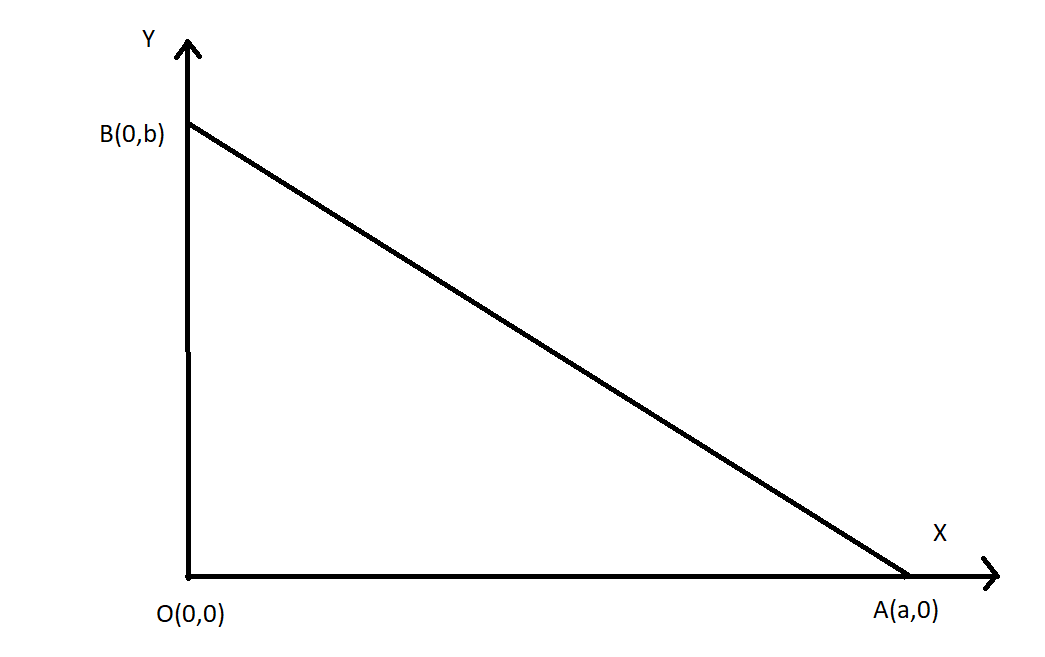
\includegraphics[width=0.8\linewidth]{triangleOAB.png}
\caption[]{}
\label{fig:ABC}
Треугольник OAB.
\end{figure}

Уравнение плоскости которому принадлежит треугольник $OAB$ имеет вид:
\begin{align}
\begin{vmatrix}
  x-0	& y-0	& z-f(O)	\\
  a		& 0		& f(A)-f(O)	\\
  0		& b		& f(B)-f(O)
\end{vmatrix}
= 0
\end{align}
Выразим координату $z$ из уравнения поверхности.
\begin{align}
z = xb(f(A)-f(O))-(ya(f(B)+f(O))+abf(O)) \div ab = \notag \\
= \frac{x}{a}(f(A)-f(O))+\frac{y}{b}(f(B)-f(O)) + f(O) \label{eq:z} \\
L_1 = \frac{x}{a}(f(A)-f(O)) \\
L_2 = \frac{y}{b}(f(B)-f(O))
\end{align}
Подставим выражение \ref{eq:z} в интеграл $\widetilde{I}$. Получим:
\begin{align}
\widetilde{I} = \iint\limits_{\triangle} L_1 dx dy+\iint\limits_{\triangle} L_2 dx dy+\iint\limits_{\triangle} f(O)= \notag \\
= \int\limits_0^a dx \int\limits_0^{b-x \frac{b}{a}} L_1 dy + \int\limits_0^b dy \int\limits_0^{a-y \frac{a}{b}} L_2 dx + ab f(O)- \frac{ab}{2}f(O) = \notag \\
= \int\limits_0^a L_1 (b-x \frac{b}{a}) dx + \int\limits_0^b L_2 (a-y \frac{a}{b}) dy + \frac{ab}{2} f(O)) = \\
= \int\limits_0^a \frac{x}{a} (f(A)-f(O)) (b-x \frac{b}{a}) dx + \notag \\
+ \int\limits_0^b \frac{y}{b} (f(B)-f(O)) (a-y \frac{a}{b}) dy + \frac{ab}{2} f(O)) =
\end{align}

\begin{align}
= \int\limits_0^a x \frac{b}{a} (f(A)-f(O)) dx - \int\limits_0^a x^2 \frac{b}{a^2} (f(A)-f(O)) dx + \notag \\
+ \int\limits_0^b y \frac{a}{b} (f(B)-f(O)) dy - \int\limits_0^b y^2 \frac{a}{b^2}(f(B)-f(O))dy + \frac{ab}{2} f(O)) = \\
= \frac{ab}{2} (f(A)-f(O)) - \frac{ab}{3} (f(B)-f(O)) + \notag \\
+ \frac{ab}{2}(f(B)-f(O)) - \frac{ab}{3} (f(B)-f(O)) + \frac{ab}{2} f(O)) = \\
= \frac{ab}{6} (f(A)-f(O)) + \frac{ab}{6} (f(B)-f(O)) + \frac{ab}{2} f(O)) = \\
= \frac{ab}{6} (f(A)+f(B)-2f(0)) + \frac{ab}{2} f(O)) = \\
= \frac{ab}{6} (f(A)+f(B)+f(0)) = \\
= \frac{ab}{2} \cdot \frac{1}{3}(f(A)+f(O)+f(B)) = \widetilde{I}
\end{align}

\begin{equation}
F_i =  \frac{1}{3}(f(A)+f(O)+f(B))
\end{equation}

\end{enumerate}

Таким образом:

\begin{align} \label{eq:Ftriangle}
F^1_{i,j} = \frac{1}{3}(f_{i,j}+f_{i,j+1}+f_{i+1,j}), \\
F^2_{i,j} = \frac{1}{3}(f_{i+1,j+1}+f_{i,j+1}+f_{i+1,j}).
\end{align}

\begin{figure}[H]
\centering
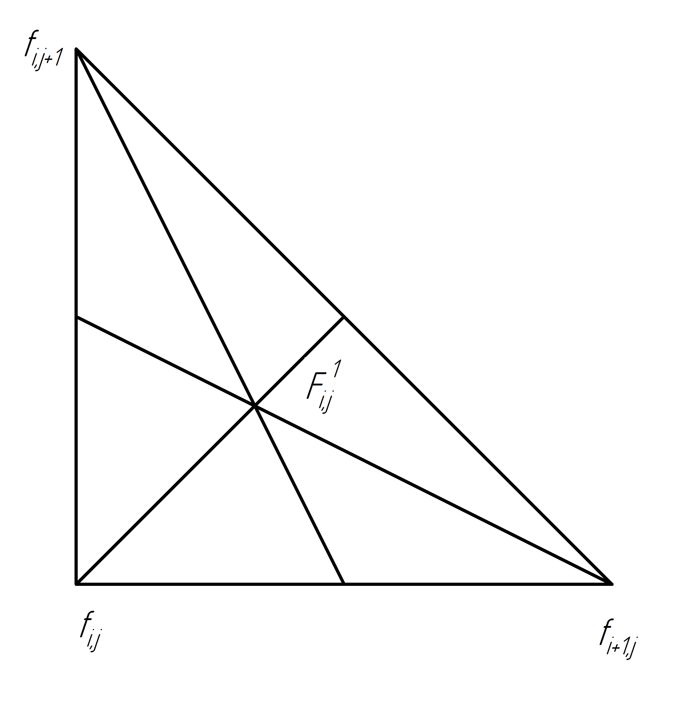
\includegraphics[width=0.8\linewidth]{median_triangle.png}
\caption{}
\label{fig:mediantriangle}
Центр тяжести треугольника.
\end{figure}

Поверхностный интеграл \ref{eq:int} будем вычислять по следующей формуле
\begin{align}\label{eq:trint}
I \approx \sum_{i=0}^{N-1} \sum_{j=0}^{M-1} I_{i,j} = \sum_{i=0}^{N-1} \sum_{j=0}^{M-1} (S_{\triangle_{i,j}^1} \cdot F_{i,j}^1 + S_{\triangle_{i,j}^2} \cdot F_{i,j}^2) = \notag \\
= \sum_{i=0}^{N-1} \sum_{j=0}^{M-1} ((h_y \cdot f_{i,j} - h_y \cdot f_{i+1,j})^2 + (h_x \cdot f_{i,j} - h_x \cdot f_{i,j+1})^2 + (h_x \cdot h_y)^2 + \notag \\
+ \frac{1}{3}(f_{i,j}+f_{i,j+1}+f_{i+1,j}) + \notag \\
+(h_y \cdot f_{i+1,j+1} - h_y \cdot f_{i+1,j})^2 + (h_x \cdot f_{i+1,j+1} - h_x \cdot f_{i,j+1})^2 + (h_x \cdot h_y)^2 + \notag \\
+\frac{1}{3}(f_{i+1,j+1}+f_{i,j+1}+f_{i+1,j}))
\end{align}
Тогда потери выхода по току по формулам (\ref{eq2}) и (\ref{eq:trint}) равны
\begin{align}\label{eq:triang}
\Delta \eta \approx (1- \eta_0) \cdot \frac{l}{S} \cdot \notag \\
\cdot \sum_{i=0}^{N-1} \sum_{j=0}^{M-1} ((h_y \cdot f_{i,j} - h_y \cdot f_{i+1,j})^2 + (h_x \cdot f_{i,j} - h_x \cdot f_{i,j+1})^2 + (h_x \cdot h_y)^2 + \notag \\
+ \frac{1}{3}(f_{i,j}+f_{i,j+1}+f_{i+1,j}) + \notag \\
+(h_y \cdot f_{i+1,j+1} - h_y \cdot f_{i+1,j})^2 + (h_x \cdot f_{i+1,j+1} - h_x \cdot f_{i,j+1})^2 + (h_x \cdot h_y)^2 + \notag \\
+\frac{1}{3}(f_{i+1,j+1}+f_{i,j+1}+f_{i+1,j})),
\end{align}
где $f_{i,j} = \frac{1}{H_{i,j}}$

\subsection{Исследование точности разработанного метода}

Для оценки полученного метода воспользуемся правилом Рунге, оценки точности \cite{litlink:samarskiy}:

\begin{equation}\label{eq:runge1}
|I-I_{\frac{h}{2}}| \approx \frac{|I_{\frac{h}{2}}-I_{h}|}{2^m-1}
\end{equation}
где $I_h$ значение полученное исследуемым методом при шаге сетки $h$, $I$ - абсолютное значение интеграла, $m$ - порядок точности исследуемого метода.

Проведём тест метода для поверхности
\begin{equation}\label{eq:surfcyl}
z(x,y) = \sqrt{4-(x-1)^2}, x \in [0,2], y \in [0,5].
\end{equation}
Она показана на рисунке \ref{fig:cylinder}.

\begin{figure}[H]
\centering
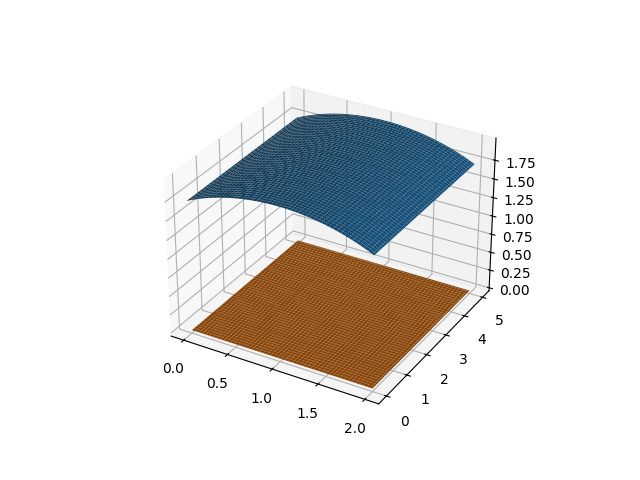
\includegraphics[width=0.8\linewidth]{cylinder.png}
\caption[]{}
\label{fig:cylinder}
\end{figure}

Возьмём подынтегральную функцию $f(x,y) = 1$, тогда интеграл можно посчитать аналитически:

\begin{equation}
I = \frac{2 \pi R}{3} = 10,471975512
\end{equation}

Значения вычисленные методом триангуляции представлены в таблице \ref{table:cylinder}.

\begin{table}
\centering
\caption{Зависимость значения $I_h$ от числа узлов\label{table:cylinder}}
\begin{tabular}{|c|c|c|c|c|}
\hline
 Число узлов	& 50		& 100		& 200		& 400		\\ 
\hline
 Значение $I_h$		& 10,471783	& 10,471927	& 10,471963	& 10,471972	\\  
\hline
\end{tabular}
\end{table}

Абсолютная погрешность считается по формуле:
\begin{equation}\label{eq:abs}
T = I-I_h.
\end{equation}

Абсолютная погрешность для поверхности заданной уравнением (\ref{eq:surfcyl}) представлена в таблице \ref{table:abspogcylinder} .

\begin{table}
\centering
\caption{\label{table:abspogcylinder}}
\begin{tabular}{|c|c|c|c|c|}
\hline
 Число узлов			& 50					& 100					& 200					& 400		\\ 
\hline
 Абсолютная погрешность & $1.92 \cdot 10^{-4}$	& $4,81 \cdot 10^{-5}$	& $1,20 \cdot 10^{-5}$	& $3,01 \cdot 10^{-6}$	\\  
\hline
\end{tabular}
\end{table}

Из (\ref{eq:runge1}) получаем:
\begin{equation}\label{eq:runge2}
m = log_2(\frac{I_{\frac{h}{2}}-I_{h}}{I-I_{\frac{h}{2}}}+1)
\end{equation}
или
\begin{equation}\label{eq:runge3}
m = log_2(\frac{I-I_{h}}{I-I_{\frac{h}{2}}}),
\end{equation}

тогда для поверхности заданной уравнением (\ref{eq:surfcyl}), $m$ принимает значения, представленные в таблице \ref{table:porTochCylinder}.

\begin{table}
\centering
\caption{\label{table:porTochCylinder}}
\begin{tabular}{|c|c|c|c|}
\hline
 Число узлов		& 50 - 100	& 100 - 200	& 200 - 400	\\ 
\hline
 Порядок точности $m$	& 2.029272	& 2.014531	& 2.007240	\\  
\hline
\end{tabular}
\end{table}

Как видно из таблицы \ref{table:porTochCylinder} порядок точности примерно равен 2.

\subsubsection*{Тест 2}

Проведём вышеописанный тест для поверхности $z = x^2$ (рис \ref{fig:squareSurf}).

\begin{figure}[H]
\centering
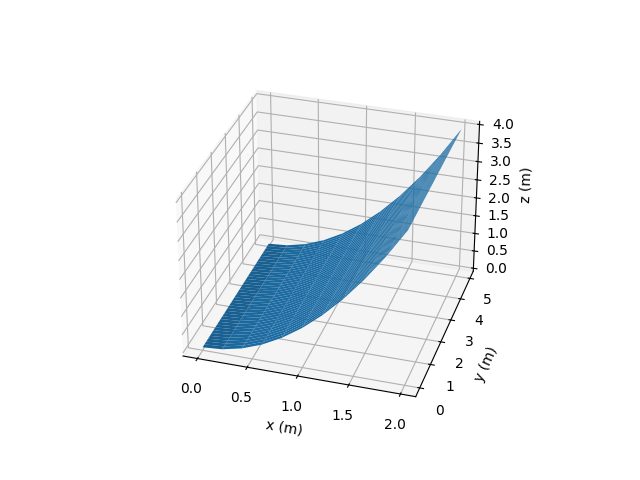
\includegraphics[width=0.8\linewidth]{squareSurf.png}
\caption[]{}
\label{fig:squareSurf}
\end{figure}

Аналитическое значение интеграла считается по формуле:

\begin{equation}
I = (\frac{ln(\sqrt{17}+4)}{4}+\sqrt{17}) \cdot 5 = 23.233919
\end{equation}

Значения посчитанные методом триангуляции показаны в таблице \ref{table:square}.

\begin{table}
\centering
\caption{\label{table:square}}.
\newline
\begin{tabular}{|c|c|c|c|c|}
\hline
 Число узлов	& 50		& 100		& 200		& 400		\\ 
\hline
 Значения		& 23.233245	& 23.233754	& 23.233878	& 23.233909	\\  
\hline
\end{tabular}
\end{table}

Порядок точности $m$ посчитаются по формуле (\ref{eq:runge2}) и представлены в таблице \ref{tablee:porTochSquare}.

\begin{table}
\centering
\caption{\label{tablee:porTochSquare}}.
\begin{tabular}{|c|c|c|c|}
\hline
 Число узлов		& 50 - 100	& 100 - 200	& 200 - 400	\\ 
\hline
 Порядок точности	& 2.029296	& 2.014537	& 2.007242	\\  
\hline
\end{tabular}
\end{table}

Порядок точности второй, аналогично тесту с поверхностью заданной уравнением (\ref{eq:surfcyl}).

Из анализ таблиц 1- 5 следует что предложенный в работе метода вычисления площади поверхности имеет второй

Ниже приводится численный расчёт значений потери по току с помощью описанного метода триангуляции.

\subsection{Вычисление коэффициента потери по току в случае поверхности раздела сред, заданной таблично.}

\subsubsection*{Пример 1}\label{ex1tr}
\addcontentsline{toc}{subsubsection}{Пример 1}
Пусть поверхность задана уравнением (\ref{eq:surf1}) (рис. \ref{fig:H1Surf}).

В формуле (\ref{eq2}) величина l соответствует минимальному расстоянию от поверхности Z до подошвы анода, $l=0.01 m$.

Значение выхода по току по формуле триангуляции (\ref{eq2}) было получено выше (\ref{eq:analit1:min}).

Проведем вычисление значений выхода по току по формуле (\ref{eq:triang}) n=k=9:
\begin{align} \label{eq:tr1min10}
\Delta \eta = 0,1 \cdot \frac{0.01}{50.000625} \int\limits_0^{10} \int\limits_0^5 \frac{\sqrt{1+(0,003)^2+(0,004)^2}}{0.44 + 0.003x + 0.004y} dy dx \approx \notag \\ \approx 0.00215165488298189
\end{align}
Аналогично вычисляется по квадратурной формуле (\ref{eq:triang}) n=k=4:
\begin{align} \label{eq:tr1min5}
\Delta \eta = 0,1 \cdot \frac{0.01}{50.000625} \int\limits_0^{10} \int\limits_0^5 \frac{\sqrt{1+(0,003)^2+(0,004)^2}}{0.44 + 0.003x + 0.004y} dy dx \approx \notag \\ \approx 0.00215168980070356
\end{align}

Результаты представленные в формулах (\ref{eq:tr1min10}) и (\ref{eq:tr1min5}) совпадают вплоть до 7 знака после запятой, что намного точнее чем по формулам (\ref{eq:sq1min10}) (\ref{eq:sq1min5}), совпадающим с точностью до 4 знака после запятой.

При этом \ref{eq:tr1min10} совпадает с аналитическим значением \ref{eq:analit1:min} с точностью до 7, а (\ref{eq:sq1min10}) совпадает с аналитическим до 4 знака.

Проведем аналогичные вычисления для другого значения l, пусть $l=0.06$ (соответствует точке на поверхности Z(x,y) в центре).

Значение выхода по току по теоретической формуле (\ref{eq2}) было получено выше (\ref{eq:analit1:med}).

Проведем вычисление значений выхода по току по формуле (\ref{eq:triang}) n=k=9:
\begin{align}\label{eq:tr1med10}
\Delta \eta = 0,1 \cdot \frac{0.06}{50.000625} \int\limits_0^{10} \int\limits_0^5 \frac{\sqrt{1+(0,003)^2+(0,004)^2}}{0.44 + 0.003x + 0.004y} dy dx \approx \notag \\ \approx 0.0129099292978913
\end{align}
Аналогично вычисляется по квадратурной формуле (\ref{eq:triang}) n=k=4:
\begin{align}\label{eq:tr1med5}
\Delta \eta = 0,1 \cdot \frac{0.06}{50.000625} \int\limits_0^{10} \int\limits_0^5 \frac{\sqrt{1+(0,003)^2+(0,004)^2}}{0.44 + 0.003x + 0.004y} dy dx \approx \notag \\ \approx 0.0129101388042213
\end{align}

Результаты представленные в формулах (\ref{eq:tr1med10}) и (\ref{eq:tr1med5}) совпадают вплоть до 4 знака после запятой, что намного точнее чем по формулам (\ref{eq:sq1med10}) (\ref{eq:sq1med5}), совпадающим с точностью до 2 знака после запятой.

При этом \ref{eq:tr1med10} совпадает с \ref{eq:analit1:med} с точностью до 6, а (\ref{eq:sq1med10}) совпадает с аналитическим до 4 знака.

Проведем вычисления для $l=0.11$ (соответствует точке на поверхности Z(x,y) в правом верхнем углу).

Значение выхода по току по теоретической формуле (\ref{eq2}) было получено выше (\ref{eq:analit1:max}).

Проведем вычисление значений выхода по току по формуле (\ref{eq:triang}) n=k=9:
\begin{align} \label{eq:tr1max10}
\Delta \eta = 0,1 \cdot \frac{0.11}{50.000625} \int\limits_0^{10} \int\limits_0^5 \frac{\sqrt{1+(0,003)^2+(0,004)^2}}{0.44 + 0.003x + 0.004y} dy dx \approx \notag \\ 0.0236682037128008
\approx
\end{align}
Аналогично вычисляется по квадратурной формуле (\ref{eq:triang}) n=k=4:
\begin{align} \label{eq:tr1max5}
\Delta \eta = 0,1 \cdot \frac{0.11}{50.000625} \int\limits_0^{10} \int\limits_0^5 \frac{\sqrt{1+(0,003)^2+(0,004)^2}}{0.44 + 0.003x + 0.004y} dy dx \approx \notag \\ 0.0236685878077391
\approx
\end{align}

Результаты представленные в формулах (\ref{eq:tr1max10}) и (\ref{eq:tr1max5}) совпадают вплоть до 5 знака после запятой, что намного точнее чем по формулам (\ref{eq:sq1max10}) (\ref{eq:sq1max5}), совпадающим с точностью до 3 знака после запятой.

При этом \ref{eq:tr1max10} совпадает с \ref{eq:analit1:max} с точностью до 5, а (\ref{eq:sq1max10}) совпадает с аналитическим до 3 знака.

Из этого можно сделать вывод, что на выбранных начальных данных метод триангуляции приближает аналитическое значение на несколько порядков лучше.

\subsubsection*{Пример 2}\label{ex2tr}
\addcontentsline{toc}{subsubsection}{Пример 2}
Пусть поверхность задана уравнением (\ref{eq:surf2}) (Рис \ref{fig:H2Surf}).

Пусть величина l соответствует минимальному расстоянию от поверхности Z до подошвы анода, $l=1 cm$.

Проведем вычисление значений выхода по току по формуле (\ref{eq:triang}) n=k=9:
\begin{align}\label{eq:tr2min10}
\Delta \eta = 0,1 \cdot \frac{0,01}{50.03007518153364} \cdot \notag \\
\cdot \int\limits_0^{10} \int\limits_0^5 \frac{\sqrt{1+0.05cos(x)cos(y)-0.05sin(x)sin(y)}}{0.44 + 0.05sin(x)cos(y)} dy dx \approx \notag \\ \approx 0.00229538198744303
\end{align}\label{eq:tr2min5}
Аналогично вычисляется по квадратурной формуле (\ref{eq:triang}) n=k=4:
\begin{align}
\Delta \eta = 0,1 \cdot \frac{0,01}{50.03007518153364}  \cdot \notag \\
\cdot \int\limits_0^{10} \int\limits_0^5 \frac{\sqrt{1+0.05cos(x)cos(y)-0.05sin(x)sin(y)}}{0.44 + 0.05 \cdot sin(x) \cdot cos(y)} dy dx \approx \notag \\ \approx 0.00229211609453886
\end{align}

Результаты представленные в формулах (\ref{eq:tr2min10}) и (\ref{eq:tr2min5}) совпадают вплоть до 5 знака после запятой, что намного точнее чем по формулам (\ref{eq:sq2min10}) и (\ref{eq:sq2min5}), совпадающим с точностью до 4 знака после запятой.

Проведем аналогичные вычисления для другого значения l, пусть $l=0.06$ (соответствует точке на поверхности Z(x,y) в точках $sin(x)=0$ или $cos(y)=0$).
Проведем вычисление значений выхода по току по формуле (\ref{eq:triang}) n=k=9:
\begin{align}\label{eq:tr2med10}
\Delta \eta = 0,1 \cdot \frac{0.06}{50.03007518153364} \cdot \notag \\
\cdot \int\limits_0^{10} \int\limits_0^5 \frac{\sqrt{1+0.05cos(x)cos(y)-0.05 sin(x)sin(y)}}{0.44 + 0.05 \cdot sin(x) \cdot cos(y)} dy dx \approx \notag \\ \approx 0.0137722919246582
\end{align}
Аналогично вычисляется по квадратурной формуле (\ref{eq:triang}) n=k=4:
\begin{align}\label{eq:tr2med5}
\Delta \eta = 0,1 \cdot \frac{0,06}{50.03007518153364} \cdot \notag \\
\cdot \int\limits_0^{10} \int\limits_0^5 \frac{\sqrt{1+0.05cos(x)cos(y)-0.05 sin(x)sin(y)}}{0.44 + 0.05 \cdot sin(x) \cdot cos(y)} dy dx \approx \notag \\ \approx 0.0137526965672332
\end{align}

Результаты представленные в формулах (\ref{eq:tr2med10}) и (\ref{eq:tr2med5}) совпадают вплоть до 4 знака после запятой, что не хуже чем по формулам (\ref{eq:sq2max10}) и (\ref{eq:sq2max5}), совпадающим с точностью до 4 знака после запятой.

Проведем вычисления для $l=0.11$ (соответствует точке на поверхности Z(x,y) на "пике").

Проведем вычисление значений выхода по току по формуле (\ref{eq:triang}) n=k=9:
\begin{align}\label{eq:tr2max10}
\Delta \eta = 0,1 \cdot \frac{0.11}{50.03007518153364} \cdot \notag \\
\cdot \int\limits_0^{10} \int\limits_0^5 \frac{\sqrt{1+0.05cos(x)cos(y)-0.05 sin(x)sin(y)}}{0.44 + 0.05 \cdot sin(x) \cdot cos(y)} dy dx \approx \notag \\ \approx 0.0252492018618734
\end{align}
Аналогично вычисляется по квадратурной формуле (\ref{eq:triang}) n=k=4:
\begin{align}\label{eq:tr2max5}
\Delta \eta = 0,1 \cdot \frac{0.11}{50.03007518153364} \cdot \notag \\
\cdot \int\limits_0^{10} \int\limits_0^5 \frac{\sqrt{1+0.05cos(x)cos(y)-0.05 sin(x)sin(y)}}{0.44 + 0.05 \cdot sin(x) \cdot cos(y)} dy dx \approx \notag \\ \approx 0.0252132770399274
\end{align}

Результаты представленные в формулах (\ref{eq:tr2max10}) и (\ref{eq:tr2max5}) совпадают вплоть до 4 знака после запятой, что намного точнее чем по формулам (\ref{eq:sq2max10}) и (\ref{eq:sq2max5}), совпадающим с точностью до 3 знака после запятой.

Анализ результатов проведенных расчетов показывает, что метод триангуляции на порядок лучше метода центральных квадратов на приведенных примерах. При этом позволяет считать интеграл на таблично заданных функциях.


\newpage
 
% даём указание на включение данного место в оглавление как секции (\section)
\addcontentsline{toc}{section}{Список литературы}
 
%далее сам список используевой литературы
\begin{thebibliography}{}
	\bibitem{litlink:kalmykov} Калмыков А.В. Математическое моделирование влияния процессов тепломассопереноса на МГД-стабильность алюминиевого электролизёра // Москва: Московский государственный университет имени М.В. Ломоносова. Факультет вычислительной математики и кибернетики. Кафедра вычислительных методов. Диссертация. 2017.
	\bibitem{litlink:bibliogr}  Белолипецкий В. М. , Пискажова Т.В. Математическое моделирование процесса электролитического получения алюминия. Решение задач управления технологией // Красноярск: Сибирский федеральный университет. Библиогр. 2013.
	\bibitem{litlink:derkach} Деркач А.С. , Левитан Г.У. , Лебедев В.И. , Сенин В.Н. , Солнцев С.С. , Форсблом Г.В. Электролиз алюминия // Издательство "Металлургия" Москва 1966.
	\bibitem{litink:AE} Grjotheim K., Rrohn C., Malinovsky. M., Matiasovsky K., Thonstad J. 2nd Edition Aluminium Electrolysys. Fundamentals of the Hall-Heroult Process. // Dusseldorf 1982.
	\bibitem{litlink:VAMI} Тепловые процессы в электролизерах и миксерах алюминиевого производства. / Под общей редакцией Громова Б. С., М.: – 1998. – С. 322.
	\bibitem{litlink:korobov} Коробов, М. А. Самообжигающиеся аноды алюминиевых электролизеров / М. А. Коробов, А. А. Дмитриев // М.: Металлургия. – 1972. – 207 с.
	\bibitem{litlink:Lillebuen}Lillebuen, B. Current Efficiency and back reaction in aluminium electrolysis // Electrochim. Acta. – 1980, V25. – P. 131– 137. 
	\bibitem{litlink:derkach2}Деркач, А. С. Влияние нестабильности тока серии на технологический режим алюминиевых электролизеров// Цветные металлы. – 1967. – № 3. – С. 39– 40.
	\bibitem{litlink:Kudryavcev}Кудрявцев Л.Д. Курс математического анализа. Том 2. // Дрофа 2004
	\bibitem{litlink:scvortsov}  Скворцов А.В., Мирза Н.С. Алгоритмы построений и анализа триангуляции // "Издательство томского университета" 2006.
	\bibitem{litlink:shirok} Широкий А.А., Аппроксимационные свойства триангуляций поверхностей // Казань 2012.
	\bibitem{litlink:samarskiy} Самарский А.А. Гулин А.В. Численные методы // Москва "Наука" 1989
\end{thebibliography}

\end{document}
